% Options for packages loaded elsewhere
\PassOptionsToPackage{unicode}{hyperref}
\PassOptionsToPackage{hyphens}{url}
%
\documentclass[
  10pt,
]{article}
\usepackage{lmodern}
\usepackage{amsmath}
\usepackage{ifxetex,ifluatex}
\ifnum 0\ifxetex 1\fi\ifluatex 1\fi=0 % if pdftex
  \usepackage[T1]{fontenc}
  \usepackage[utf8]{inputenc}
  \usepackage{textcomp} % provide euro and other symbols
  \usepackage{amssymb}
\else % if luatex or xetex
  \usepackage{unicode-math}
  \defaultfontfeatures{Scale=MatchLowercase}
  \defaultfontfeatures[\rmfamily]{Ligatures=TeX,Scale=1}
\fi
% Use upquote if available, for straight quotes in verbatim environments
\IfFileExists{upquote.sty}{\usepackage{upquote}}{}
\IfFileExists{microtype.sty}{% use microtype if available
  \usepackage[]{microtype}
  \UseMicrotypeSet[protrusion]{basicmath} % disable protrusion for tt fonts
}{}
\makeatletter
\@ifundefined{KOMAClassName}{% if non-KOMA class
  \IfFileExists{parskip.sty}{%
    \usepackage{parskip}
  }{% else
    \setlength{\parindent}{0pt}
    \setlength{\parskip}{6pt plus 2pt minus 1pt}}
}{% if KOMA class
  \KOMAoptions{parskip=half}}
\makeatother
\usepackage{xcolor}
\IfFileExists{xurl.sty}{\usepackage{xurl}}{} % add URL line breaks if available
\IfFileExists{bookmark.sty}{\usepackage{bookmark}}{\usepackage{hyperref}}
\hypersetup{
  hidelinks,
  pdfcreator={LaTeX via pandoc}}
\urlstyle{same} % disable monospaced font for URLs
\usepackage[top=0cm, margin=1.8cm, left=1cm, right=1cm]{geometry}
\usepackage{graphicx}
\makeatletter
\def\maxwidth{\ifdim\Gin@nat@width>\linewidth\linewidth\else\Gin@nat@width\fi}
\def\maxheight{\ifdim\Gin@nat@height>\textheight\textheight\else\Gin@nat@height\fi}
\makeatother
% Scale images if necessary, so that they will not overflow the page
% margins by default, and it is still possible to overwrite the defaults
% using explicit options in \includegraphics[width, height, ...]{}
\setkeys{Gin}{width=\maxwidth,height=\maxheight,keepaspectratio}
% Set default figure placement to htbp
\makeatletter
\def\fps@figure{htbp}
\makeatother
\setlength{\emergencystretch}{3em} % prevent overfull lines
\providecommand{\tightlist}{%
  \setlength{\itemsep}{0pt}\setlength{\parskip}{0pt}}
\setcounter{secnumdepth}{-\maxdimen} % remove section numbering
\usepackage{titlesec}
\usepackage{fontspec}
\usepackage{fancyhdr}
\setmainfont{montserrat}
\usepackage{xcolor}
\usepackage{array}
\usepackage[document]{ragged2e}
\definecolor{p1}{HTML}{088A08}
\definecolor{t1}{HTML}{088A08}
\titleformat{\section}{\Large\fontsize{13}{13}\bfseries\sffamily\color{t1}}{}{0pt}{}
\pagestyle{fancy}
\fancyhf{}
\fancyhead[C]{\color{p1}{\changefont\textbf{GEOMAR PERALES APAICO}}}
\fancypagestyle{plain}{\pagestyle{fancy}}
\usepackage{titling}
\usepackage{setspace}
\usepackage{float} - \usepackage{tabularx}
\ifluatex
  \usepackage{selnolig}  % disable illegal ligatures
\fi

\author{}
\date{\vspace{-2.5em}}

\begin{document}

\newcommand{\changefont}{%
    \fontsize{16}{9}\selectfont
}

\newpage

\begin{figure}[tph]
\begin{minipage}[t]{0.3\textwidth}
  \centering
  \vspace*{-6\baselineskip}
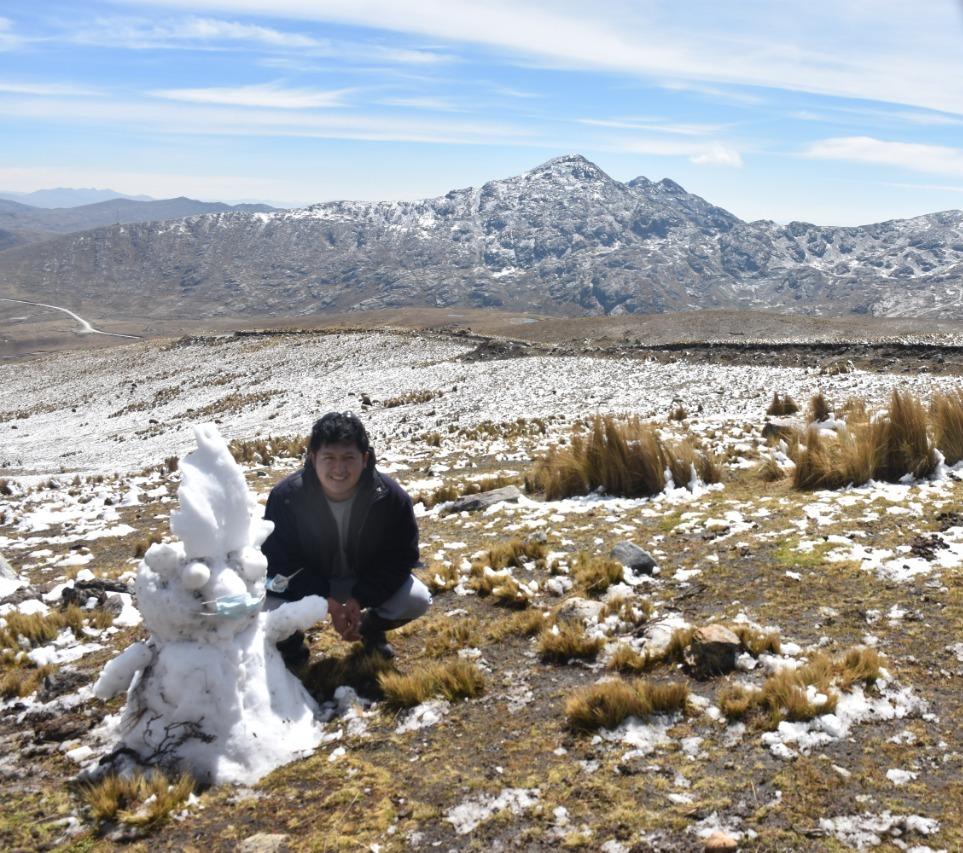
\includegraphics[width=5.0cm]{images/gperales.jpg}
  \section{PERFIL\vspace{-0.35em}}
  \justify

Estoy enfocado a las áreas de Hidrología, Hidráulica y Recursos Hídricos, tengo 
buen desempeño para el trabajo en equipo y la mejora continua.
\setlength\parskip{1em}

Tengo capacidades técnicas en: Hidrología, procesando y analizando datos usando R,
Python y Excel; En Recursos hídricos, recopilando y procesando información hídrica;
en Hidráulica, desarrollando modelos de simulación.

\setlength\parskip{1em}

Uno de mis objetivos es cursar la maestría de Hidroinformática en Delft (Holanda),
para lo cual llevo una preparación autodidacta técnica, cultural y bilingüe.

  \subsection{IDIOMAS\vspace{0em}}

\textcolor{darkgray}{\textbf{Español - nativo}\vfill\vspace{-1mm}}
\textcolor{darkgray}{\textbf{Quechua - Básico (en proceso)}\vfill\vspace{-1mm}}
\textcolor{darkgray}{\textbf{Inglés- Básico (en proceso)}\vfill\vspace{-1mm}}

  \subsection{REFERENCIAS\vspace{0em}}

\raggedright
{Ing. Gustavo Atúncar\vfill\vspace{-3mm}}
{Esp. de Hidrología e Hidráulica\vfill\vspace{-3mm}}
{Cel. N° 939272465\vfill\vspace{0mm}}

{Ing. Yonatan Bustamante\vfill\vspace{-3mm}}
{Esp. de Hidrología e Hidráulica\vfill\vspace{-3mm}}
{Cel. N° 982267689\vfill\vspace{0mm}}

{Ing. Elvis Castro\vfill\vspace{-3mm}}
{Jefe de Recursos Hídricos, SRK\vfill\vspace{-3mm}}
{Cel. N° 956302303\vfill\vspace{0mm}}


\vspace{1mm}

  \end{minipage}
  %
  \hfill
  %
  \begin{minipage}[t]{0.65\textwidth}
  \justify
  \vspace*{-6\baselineskip}

\section{TITULACIÓN UNIVERSITARIA\vspace{-0.35em}}

\textcolor{black}{\textbf{Bachiller en Ing. Mecánica de Fluidos | Marzo - 2020}}
\vspace{1.3mm}\vfill
\textcolor{black}{\textbf{Formación en Ing. Mecánica de Fluidos | Julio - 2019}}
\vspace{1.3mm}\vfill
Universidad Nacional Mayor de San Marcos (UNMSM)
\vspace{0.6mm}\vfill
- Formación en Recursos Hídricos, Hidrología e Hidráulica.
\vspace{0.6mm}\vfill

\section{FORMACIÓN COMPLEMENTARIA\vspace{-0.35em}}

- Hidrología General: 40 h| Agencia Nacional de Aguas| MOOC, Brasil\vspace{0.7mm}\vfill
- Especialización en R: Básico, Intermedio y Avanzado: 84 h| SDC\vspace{0.7mm}\vfill
- Modelos de Gestión de Recursos Hídricos: WEAP Y MODFLOW: 40 h| TYPSA\vspace{0.7mm}\vfill
- Dipl. de Mod. Hidráulico e Hidrológico: 120 h| CIDHMA\vspace{0.7mm}\vfill
- Gestión de Proy. con Metodologías Agiles: 40 h| Univ. Telefónica| MOOC, España\vspace{0.7mm}

\section{SKILLS\vspace{-0.35em}}

\textcolor{black}{\textbf{MODELAMIENTO}}


\begin{center}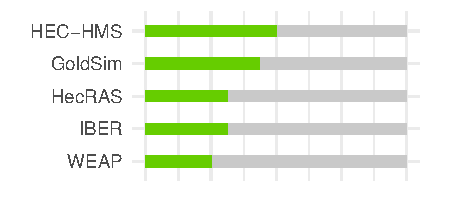
\includegraphics{resume_v05a_files/figure-latex/unnamed-chunk-1-1} \end{center}

\textcolor{black}{\textbf{CAD Y SIG}}


\begin{center}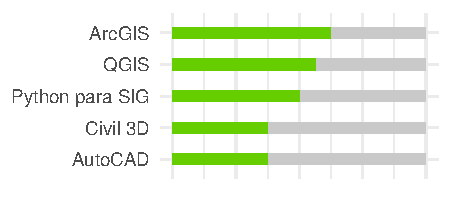
\includegraphics{resume_v05a_files/figure-latex/unnamed-chunk-2-1} \end{center}

\textcolor{black}{\textbf{ESTADÍSTICA Y LENG. DE PROGRAMACIÓN}}

\begin{center}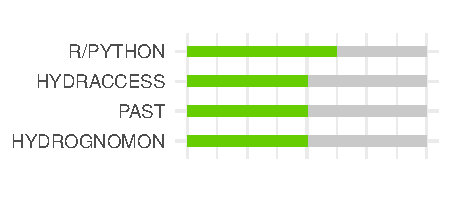
\includegraphics{resume_v05a_files/figure-latex/unnamed-chunk-3-1} \end{center}

  \end{minipage}
\end{figure}

\pagebreak

\textbackslash begin\{document\} \newpage \centering

~begin\{tabular\}{[}H{]}\{ m\{15em\} \textbar{} m\{39em\} \textbar{} \}
cell1 \&
ffffffffffffffffffffffffffffffffffffffffffffffffffffffffffffffffffff\\
ffffff fffffff fffffffff ffff fffff ffff
fffffffffffffffffffffffffffffffff \textbackslash{} cell4 \& cell5
\textbackslash{}\\
cell7 \& cell8 \}

\textbackslash end\{tabular\}

\textbackslash end\{document\}

\newpage
\centering
  \begin{tabular}{ c c c }
  
 cell1 & cell2 & cell3 \\ 
 cell4 & cell5 & cell6 \\  
 cell7 & cell8 & cell9   
 
 
  \end{tabular}

\end{document}
